% !BIB program = bibtex
%%%%%%%%%%%%%%%%%%%%%%%%%%%%%%%%%%%%%%%%%%%%%%%%%%%%%%%
%%% LATEX FORMATTING - LEAVE AS IS %%%%%%%%%%%%%%%%%%%%
\documentclass[11pt]{article} % documenttype: article
\usepackage[top=20mm,left=20mm,right=20mm,bottom=15mm,headsep=15pt,footskip=15pt,a4paper]{geometry} % customize margins
\usepackage{times} % fonttype
\usepackage{csquotes}
\usepackage{graphicx}
\usepackage[backend=bibtex, sorting=none]{biblatex}

\addbibresource{shifei_chen_assignment_3.bib}
\graphicspath{ {./images/} }

\makeatletter         
\def\@maketitle{   % custom maketitle 
\begin{center}
{\bfseries \@title}
{\bfseries \@author}
\end{center}
\smallskip \hrule \bigskip }

%%%%%%%%%%%%%%%%%%%%%%%%%%%%%%%%%%%%%%%%%%%%%%%%%%%%%%%%%%%%%%%%%%%%
%%% MAKE CHANGES HERE %%%%%%%%%%%%%%%%%%%%%%%%%%%%%%%%%%%%%%%%%%%%%%
\title{{\LARGE Natural Language Processing: Assignment 3}\\[1.5mm]} % Replace 'X' by number of Assignment
\author{Shifei Chen} % Replace 'Firstname Lastname' by your name.

%%%%%%%%%%%%%%%%%%%%%%%%%%%%%%%%%%%%%%%%%%%%%%%%%%%%%%%%%%%%%%%%%%%%
%%% BEGIN DOCUMENT %%%%%%%%%%%%%%%%%%%%%%%%%%%%%%%%%%%%%%%%%%%%%%%%%
%%% From here on, edit document. Use sections, subsections, etc.
%%% to structure your answers.
\begin{document}
\maketitle

\section{Dependency Annotation}

Here are three typical errors I have made during my manual annotation.

\subsection{\texttt{nmod} vs \texttt{compound}}

\begin{displayquote}
  "If a Turkish employee quits, then the Turkish work councils come."
\end{displayquote}

The ambiguation between a single \texttt{nmod} and a \texttt{compound} noun is confusing to me. In the phrase "work councils" I have annotated "work" as a nominal modifier to "councils" while the golden standard says they should be compounded. A compound word usually consists of nouns (or verbs, adjectives, etc.) being writted closely to each other. In fact they are so close that in some Language like Swedish people usually write them together, without whitespaces. Meanwhile a nominal modifier is usually used to describe an attribute or genitive complement\cite{NmodUD}. In this case, "work" can be argued to be the attribute of "councils" but since this is an idiom\cite{WorksCouncilWiki} so I prefer the golden standard.

\subsection{\texttt{mark}}

\begin{displayquote}
  "National reaction to the events in Kansas demonstrated how deeply divided the country had become."
\end{displayquote}

Here I have marked the word "how" as a \texttt{mark} to the head word "become" rather than an \texttt{advmod} to the head word "deeply". It is clear that in this sentence, "how deeply divided the country had become" is a complement clause, acting as the object to the verb "demonstrated". The word "become" is a \texttt{ccomp} to "demonstrated"\cite{CcompUD}. The clause does clearly indicate that its object is "divided", not "how", hence we should consider "how" as an adverbial modifer to the other adverb "deeply", even though sometimes "how" can be the mark word of a complement clause\cite{MarkUD}.

\subsection{Subjects in Passive Voice}

\begin{displayquote}
  "The RHS collected comments sent in by schoolchildren and teachers involved in the experiment."
\end{displayquote}

I annotated "sent" to be the clause modifier of noun (\texttt{acl}) to "collected" and "schoolchildren" to be the nominal subject of "comments". The error in the former situation is pretty obvious since "collected" is a verb\cite{AclUD}. I should have annotated "sent" to be the \texttt{acl} of "comments". The latter is also wrong. Judging by the meaning, it may be intriguing to annotate "schoolchildren" as a \texttt{nsubj} because those children are the one who sent comments. But there is an example from Universal Dependency which explicly says "(\texttt{obl} is used) for the agent of a passive verb (with the optional subtype \texttt{obl:agent}):"\cite{OblUD}. We should mark "schoolchildren" as the \texttt{obl} to the verb "sent".

\section{Dependency Parsing}

Below are two examples of errors made by the parser in Lab 9.

\begin{displayquote}
  A witness told police that the victim had attacked the suspect in April.
\end{displayquote}

In this sentence my parser annotated "police" as the \texttt{obj} of the verb "told", which should be an \texttt{iobj}. "Tell" can have a direct object like in the verb phrase "tell a lie" but here "police" is not the subject. In fact, the clause beginning with "that" is the real subject. This might be caused by our corpus containing too many "tell"s having direct objects, or by the fact the our parser, as a transition based parser, always has a limited scope of words--it can't foresee the words behind "police" therefore it prefers "tell" to have a direct object. Nevertheless UD has a specific label \texttt{iobj} for this kind of indirect subject\cite{IobjUD} and we should stick to that.

The problem of limited scope of words can also be demonstrated by the other example in Figure 1.

\begin{figure}[ht]
  \centering
  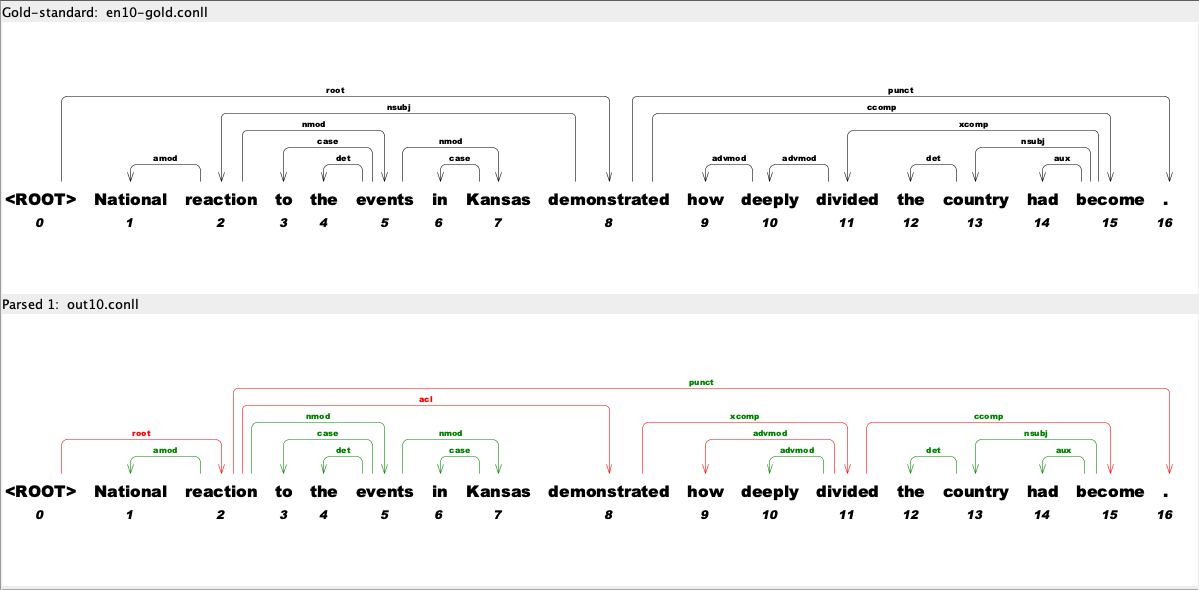
\includegraphics[width=0.9\textwidth]{images/figure_limited_scope.png}
  \caption{The Problem of Limited Scope}
\end{figure}

My parser mistook the main structure of the sentence: it believed "reaction" is the root therefore it continued to make further mistakes, which I believe is the case of "error propagation". It had to do some greedy "reduce" step in order to release some space in its stack, especially for sentences which the root word is located in the further back.

A transition based depnedency parser has three elements: a stack $S$, a buffer $B$ for unprocessed words and a list $A$ for arcs it has built. Starting with the root word in $S$, it scans the sentence from left to write and makes predictions learned from machine learning about whether to build a left arc or a right arc, to pop the top word in the stack (reduce) or to push a word from the buffer to the stack (move). The termination point is when the parser empties its buffer and at that time $A$ is the complete list of parsed arcs.

We shall look at this sentence as an example to show how the parser works.

\begin{equation}
  [\texttt{ROOT}]_s [\texttt{He worked for the BBC for a decade .}]_B
\end{equation}
We start with root being our $W_0$.
\begin{equation}
  [\texttt{ROOT He}]_s [\texttt{worked for the BBC for a decade .}]_B
\end{equation}
Shift "He" into $S$
\begin{equation}
  [\texttt{ROOT}]_s [\texttt{worked for the BBC for a decade .}]_B
\end{equation}
Build a left arc from "worked" to "He", label it \texttt{nsubj}.
\begin{equation}
  [\texttt{ROOT worked}]_s [\texttt{for the BBC for a decade .}]_B
\end{equation}
Build a right arc from root to "worked", label it \texttt{ROOT}.
\begin{equation}
  [\texttt{ROOT worked for the}]_s [\texttt{the BBC for a decade .}]_B
\end{equation}
Shift "for" and the.
\begin{equation}
  [\texttt{ROOT worked for}]_s [\texttt{BBC for a decade .}]_B
\end{equation}
Build a left arc from "BBC" to "the", label it \texttt{det}.
\begin{equation}
  [\texttt{ROOT worked}]_s [\texttt{BBC for a decade .}]_B
\end{equation}
Build a left arc from "BBC" to "for", label it \texttt{case}.
\begin{equation}
  [\texttt{ROOT worked BBC}]_s [\texttt{for a decade .}]_B
\end{equation}
Build a right arc from "worked" to "BBC", label it \texttt{obl}.
\begin{equation}
  [\texttt{ROOT worked BBC for a}]_s [\texttt{decade .}]_B
\end{equation}
Shift "for" and "a".
\begin{equation}
  [\texttt{ROOT worked BBC for}]_s [\texttt{decade .}]_B
\end{equation}
Build a left arc from "decade" to "a", label it \texttt{det}.
\begin{equation}
  [\texttt{ROOT worked BBC}]_s [\texttt{decade .}]_B
\end{equation}
Build a left arc from "decade" to "for", label it \texttt{case}.
\begin{equation}
  [\texttt{ROOT worked}]_s [\texttt{decade .}]_B
\end{equation}
Reduce "BBC".
\begin{equation}
  [\texttt{ROOT worked decade}]_s [\texttt{.}]_B
\end{equation}
Build a right arc from "worked" to "decade", label it \texttt{obl}.
\begin{equation}
  [\texttt{ROOT worked}]_s [\texttt{.}]_B
\end{equation}
Reduce "decade".
\begin{equation}
  [\texttt{ROOT worked .}]_s []_B
\end{equation}
Build a right arc from "worked" to ".", label it \texttt{punc}. The empty buffer $B$ marks our end of parsing.

\printbibliography

\end{document}
